\chapter{Methodology}  \label{sec:method}
The \ac{dea} is a new attack method that extends the capabilities of \ac{gma}s by going beyond the intersection of datasets and attempting to re-identify previously unmapped individuals.
This chapter details the methodology behind the \ac{dea}, including the necessary modifications to the \ac{gma}, the design and implementation of the \ac{dea} itself, and the role of \ac{ann}s in enabling probabilistic reconstruction of \ac{pii} from encoded data.

The \ac{dea} builds upon the \ac{gma} by utilizing its re-identification results as a foundation for further inference.
Since the \ac{gma} only re-identifies matches between records that exist in both the attacker’s dataset and the encoded target dataset, it can leave a significant portion of records encoded.
The goal of the \ac{dea} is to extend this re-identification process by leveraging a machine learning based approach to infer missing \ac{pii} by training an \ac{ann}.

To achieve this, the \ac{dea} follows a structured pipeline consisting of several key steps as can be seen in Figure~\ref{fig:deaoverview}.
First, the results of the \ac{gma} are extracted in a predefined format to serve as training data for the \ac{ann}.
These results include re-identified individuals, their corresponding encoded representations, and the plaintext information that were successfully mapped.
Additionally the results include the not re-identified individuals with just the encoded \ac{pii}.
Ensuring a structured and consistent format is crucial, as it allows for seamless integration into the subsequent processing stages.

\begin{figure}[H]
    \centering
    \includegraphics[width=0.7\textwidth, page=14]{img/visualization.pdf}
    \caption{Overview of the \ac{dea} attack pipeline.}
    \label{fig:deaoverview}
  \end{figure}

Once the data is extracted, it is transformed into a format suitable for \ac{ann} training.
This involves setting up specialized datasets that convert encoded representations and their corresponding labels, which are plaintext n-grams, into tensor-based formats that can be efficiently processed by deep learning models.
The dataset is then split into training, validation, and test sets, and respective data loaders are created to facilitate efficient batch processing during training.

With the data pipeline in place, a \ac{ann} is designed to perform multi-label classification, predicting the likelihood of individual n-grams occurring in an encoded record.
The architecture consists of an input layer that receives the encoded representation, a series of hidden layers that learn complex patterns within the data, and an output layer that produces probability scores for all possible n-grams.
To optimize performance, an appropriate loss function and optimizer are selected, ensuring stable convergence during training.
The model is trained using the training set while the validation set is used to monitor performance and prevent overfitting.

Once the \ac{ann} is trained, it is applied to the set of not-reidentified individuals, i.e., records that remained unmapped after the \ac{gma}.
The model outputs a probability distribution for each possible n-gram of each entry, indicating the likelihood of its presence in the corresponding plaintext data.
To refine these predictions, a thresholding mechanism is applied, filtering out low-confidence predictions and retaining only the most relevant n-grams.
Finally, the predicted n-grams are aggregated and reconstructed into potential \ac{pii}, forming the final step of the \ac{dea} process.

This methodological approach represents a significant step forward in attacking \ac{pprl} systems.
By leveraging deep learning techniques, the \ac{dea} enables an attacker to infer sensitive personal information beyond the scope of traditional \ac{gma} approaches.
The following sections provide an in-depth discussion of each component, including the design choices, implementation details, and challenges encountered during development.

\section{Modifications to the \ac{gma}} \label{sec:modifications}

The \ac{gma} serves as the foundation for the \ac{dea} by providing the initial set of re-identified individuals along with their corresponding encodings and the remaining non-reidentified individuals.
The effectiveness of the \ac{dea} is directly dependent on the performance of the \ac{gma}.
A higher re-identification rate in the \ac{gma} results in a larger training dataset for the \ac{dea}, which improves its ability to infer missing n-grams and reconstruct additional identities.
Conversely, if the \ac{gma} has a low re-identification rate, the \ac{dea} is constrained by the limited amount of labeled training data, reducing its overall effectiveness in identifying individuals beyond the \ac{gma}.

To integrate the \ac{gma} as a preprocessing step for the \ac{dea}, modifications were made to the original implementation by Schaefer et al \cite{schaefer2024}.
While the core algorithm remains unchanged, adjustments were necessary to ensure that the \ac{gma} outputs results in a structured format that facilitates the training of the \ac{ann} used in the \ac{dea}.
Originally, the \ac{gma} only provided a simple mapping between IDs of re-identified individuals.
However, for the \ac{dea} to be able to learn meaningful patterns, it requires access to both the plaintext \ac{pii} and their corresponding encodings.
Therefore, modifications were implemented to ensure that the \ac{gma} outputs data in two sets in the following format:

\begin{itemize}
    \item For re-identified individuals: \texttt{<\ac{pii}> <encoding> <uid>}
    \item For not-reidentified individuals: \texttt{<encoding> <uid>}
\end{itemize}

Here, the uid is included only for research and testing purposes.
It allows the researcher to manually track individuals across different processing stages.
However, in a real-world attack scenario, these uids are neither available nor necessary.
They are entirely excluded from any \ac{dea} training or inference steps, ensuring that the attack methodology remains realistic and applicable in practical settings.

In addition to formatting adjustments, some components of the \ac{gma} were removed to streamline the process and reduce unnecessary complexity.
Specifically, encoding schemes besides the \ac{tsh}, \ac{tmh} and \ac{bf} were excluded, as the focus of the \ac{dea} remains on these.
Other not required components were also removed, such as the graph visualizations and benchmark tests focusing on the \ac{gma} itself.
This decision was taken as the \ac{gma} is not focus of this research paper and its validty and performance is given by previous research.
These optimizations resulted in a leaner and more efficient attack pipeline, reducing computational overhead while retaining all essential functionality.

With these modifications in place, the starting point for the \ac{dea} is clearly defined.
The attack begins with two structured datasets:

\begin{enumerate}
    \item Re-identified individuals, containing both their plaintext \ac{pii} and corresponding encodings, formatted as described above.
    \item Not-reidentified individuals, for whom only the encodings are available, serving as the primary targets for inference using the \ac{dea}.
\end{enumerate}

By leveraging this structured output, the \ac{dea} is able to train a machine learning model capable of probabilistically reconstructing missing n-grams from the encoded records of not-reidentified individuals.
The following sections will detail the implementation of this approach, including dataset preparation, model architecture, and evaluation strategies.

\section{Design and Implementation of the \ac{dea}} \label{sec:designandimplementation}

The \ac{dea} aims to reconstruct plaintext \ac{pii} from encoded records by leveraging machine learning techniques.
This section provides a detailed account of the problem definition, data representation, \ac{ann} architecture, and training methodology.
A key challenge in the implementation of the \ac{dea} is the diversity of encoding schemes used to protect sensitive data.
Since different encoding methods transform plaintext into distinct numerical representations, the design of the \ac{dea} must account for these variations by tailoring the dataset structure and \ac{ann} architecture to each encoding scheme.

To address this challenge, the \ac{dea} follows a modular approach, where the general attack methodology remains consistent, but specific implementations are adapted for each encoding scheme.
While the input representation and network architecture differ based on the encoding method, the output format remains uniform across all models.
The attack is formulated as a multi-label classification problem, where the \ac{ann} predicts the probability of individual n-grams being present in the original \ac{pii}.
For each encoding scheme, a dedicated dataset structure is constructed to transform encoded records into an appropriate numerical format suitable for \ac{ann} training.
Additionally an own \ac{ann} structure is considered for each encoding scheme, ensuring that the model can effectively learn the mapping between encoded values and plaintext n-grams.

\subsection{Problem Definition} \label{sec:problemdefinition}

The primary challenge that the \ac{dea} seeks to address is the limited scope of re-identifications achieved by the \ac{gma}.
While the \ac{gma} is effective in linking records by exploiting the structural relationships within encoded datasets, its success is inherently constrained to individuals who are present in both datasets, plain and encrypted, and can be matched based on graph similarity.
However, in many real-world scenarios, there exists additional re-identification potential beyond these direct matches.

One possible approach to extending re-identifications is to extend the \ac{gma} by using additional publicly available data and rerun the \ac{gma} in an iterative manner, gradually refining the matching process.
However, this approach is inherently dependent on external data sources and may not be viable in cases where such additional information is scarce.
Instead, the \ac{dea} introduces a novel method that reconstructs deterministic relationships between encoded representations and their corresponding plaintext information, leveraging the fact that all encoding schemes used in \ac{pprl} rely on hash functions or some other determinstic mapping.

Hash functions as an example provide a fixed-length output for an arbitrary-length input, and crucially, they are deterministic, meaning that the same input will always produce the same output.
The \ac{dea} exploits this property by training \ac{ann}s to learn statistical relationships between the encoded values and the original n-grams of \ac{pii}.
The goal is to recover the most probable plaintext representation given an encoded input, effectively treating the attack as a probabilistic frequency-based inference problem.
However, several factors make this task difficult.

The first challenge is that the exact number and type of hash functions used in the encoding process are unknown.
This means that the model must learn patterns without explicit knowledge of the hashing mechanisms applied.
Fortunately, this limitation is mitigated by the fact that the \ac{dea} does not require a one-to-one mapping between hash outputs and plaintext but instead relies on statistical inference across multiple samples.

A more fundamental issue arises from the collision property of hash functions.
Since hash functions map an infinite input space to a finite output space, different inputs may produce identical hashes, making it difficult to perfectly recover the original plaintext values.
These collisions introduce inherent uncertainty into the re-identification process, preventing the \ac{dea} from achieving perfect performance.
As a result, the \ac{dea}'s predictions are probabilistic rather than deterministic, meaning that the attack can estimate the likelihood of a given n-gram being present in the original \ac{pii} but cannot guarantee absolute correctness.

The primary reason the \ac{gma} alone fails to achieve this kind of re-identification is that it relies solely on the structural properties of the dataset, without attempting to infer direct relationships between encoded values and their plaintext counterparts.
By contrast, the \ac{dea} extends the capabilities of the \ac{gma} by reconstructing individual plaintext components from encoded representations, thereby increasing the overall re-identification potential.
This novel approach significantly enhances the attack's effectiveness, allowing for the possibility of re-identifying individuals who were previously considered unmatchable using traditional graph-based techniques.

\subsection{Data Representation} \label{sec:representation}

For a \ac{ann} to function effectively and achieve successful results, it is essential to preprocess the data into a format that is consumable by deep learning models.
This preprocessing applies to both input data, which consists of encoded representations of \ac{pii}, and output data, which represents labels as the predicted n-grams.
Since \ac{ann}s in PyTorch operate on tensor representations, the transformation of encoded records into tensors is a crucial step.
This transformation ensures that both re-identified and not-reidentified individuals are structured in a way that facilitates efficient training and inference.
To achieve this, PyTorch datasets are created to handle the conversion of encoded inputs into tensors while also encoding the expected output in a suitable multi-label classification format.

The data structure follows the encoding schemes previously described, with different encoding methods leading to different preprocessing techniques.
Each encoding method requires a tailored transformation into tensors, ensuring compatibility with the \ac{ann} architecture while preserving as much information as possible.

\subsubsection{\ac{bf} Encoding}
\ac{bf}s are fixed-length binary strings, with their length determined by Alice’s chosen parameters.
These bitstrings are converted into PyTorch tensors of the same length.
The transformation is rather straightforward, each bit in the \ac{bf} is mapped directly to the tensor, with the positions of 1-bits preserved, ensuring that the structure of the encoding remains unchanged.
The resulting tensor has the same length as the \ac{bf}, with ones at positions where bits were set in the original filter and zeros elsewhere.

\subsubsection{\ac{tmh} Encoding}
\ac{tmh}, like \ac{bf}s, also produces fixed-length binary bitstrings, where the length depends on the parameters chosen by Alice.
The transformation process follows the same principles as for \ac{bf}s: each \ac{tmh} bitstring is converted into a PyTorch tensor of equal length, preserving the positions of the 1-bits.
This ensures that the \ac{ann} receives the \ac{tmh} encoding as a structured binary representation.

\subsubsection{\ac{tsh} Encoding}
The preprocessing of \ac{tsh} encodings is more complex due to its variable-length representation.
Unlike \ac{bf} and \ac{tmh}, \ac{tsh} does not produce fixed-length binary bitstrings but rather a set or list of integers with the size of the set being of arbitrary size.
This arbitrary size is caused as columns with only zero values are dropped during the \ac{tsh} encoding process.

However, \ac{ann}s require fixed-length input vectors, meaning that an appropriate transformation must be applied.
Aggregation techniques (such as computing averages) would lead to information loss, which is undesirable in this limited-knowledge setting.
Instead, two different approaches are considered for transforming \ac{tsh} into a tensor-compatible format:

\texttt{Padding Approach}
The first method involves determining the largest set size among all \ac{tsh}-encoded records.
This value can also be derived from the chosen parameters by Alice as they are known by the linkage unit (i.e. they can be inferred).
This maximum length is then used to define a fixed-size tensor representation for all samples.
Each set of \ac{tsh} integers is mapped into a tensor where the original values are placed at the beginning, and any remaining positions are padded with zeros.
For example, if the largest set size is 5, and two different \ac{tsh} sets are `{22, 3, 4}` and `{11, 8}`, they are transformed into `[22, 3, 4, 0, 0]` and `[11, 8, 0, 0, 0]`, respectively.
This causes loss of information as the position of integers, produced during hashing at the index of the columns, can not be considered.

\texttt{Frequency String Approach}
The second method transforms the \ac{tsh} encoding into a bitstring format similar to \ac{bf} and \ac{tmh}.
In this case, the maximum integer value encountered in any \ac{tsh} encoding (e.g., 12345 if that is the highest number present) determines the tensor length.
Each \ac{tsh} integer is then mapped to a corresponding index, setting that position in the tensor to 1.
If a specific value appears multiple times within a \ac{tsh} set, the corresponding index in the tensor is incremented instead of simply being set to 1.
This ensures that frequency information is retained, reducing the risk of losing critical details due to hash collisions.
For instance, if `22` appears twice in a \ac{tsh} encoding, the tensor at index `22` will have the value 2 rather than 1.
This approach ensures that the \ac{ann} receives a structured input that captures the frequency of each integer value within the \ac{tsh} set and whether it occurs or not.

Regardless of the encoding scheme used, the output of the \ac{ann} remains the same.
The goal is to map the encoding input to the probability distribution of n-grams, which means that the output layer always predicts the likelihood of each possible n-grams being present in the original plaintext.

\subsection{Re-Identified Individuals as Labeled Training Data}

To enable supervised learning, re-identified individuals are used as labeled training data.
Since their \ac{pii} is known along with their corresponding encoded representation, it is possible to create a training dataset where the input consists of transformed encodings (\ac{bf}, \ac{tmh}, or \ac{tsh}) and the output consists of the correct n-grams derived from the original \ac{pii}.

To facilitate this process, a predefined dictionary of all possible n-grams is constructed. This dictionary includes:
\begin{itemize}
   \item Alphabetical n-grams (e.g. for 2-grams `aa` to `zz`)
   \item Numerical n-grams (e.g. for 2-grams `00` to `99`)
   \item Mixed alphanumeric n-grams (e.g. for 2-grams `a0` to `z9`)
\end{itemize}

Since the datasets used in this research primarily contain first names, last names, and birthdates, these character sets cover the majority of cases.
Each possible n-grams is mapped to a specific index in the output tensor, ensuring a consistent representation across training samples.
For example, if index `1` corresponds to the 2-gram \enquote{ab}, and the \ac{ann} predicts a 60\% probability at index 1, this is interpreted as a 60\% likelihood that \enquote{ab} was present in the original plaintext.

By structuring the data in this way, the \ac{ann} is trained to map the encoding to its corresponding n-grams representation, ultimately enabling the \ac{dea} to probabilistically reconstruct the original \ac{pii} from encoded data.

\subsection{\ac{ann} Architecture for \ac{dea}} \label{sec:architecture}

Attempting to reconstruct plaintext information from encoded representations based on hash functions presents a significant challenge due to the nature of cryptographic hashing.
Since hash functions are designed to be one-way functions, reversing the transformation to recover the original input is theoretically infeasible.
However, while exact reconstruction is not possible, a probabilistic approach can still be applied to infer likely plaintext components based on patterns in the encoded data.

\ac{ann}s provide a powerful framework for learning complex mappings between input encodings and output predictions, making them well-suited for this task.
The function of the \ac{ann} in the \ac{dea} is to predict n-grams by learning from re-identified individuals, individuals whose plaintext information is known along with their corresponding encoding.
Through this learning process, the model captures frequency patterns that emerge due to the deterministic properties of hash functions.
In essence, the \ac{ann} learns which n-grams are mapped to specific positions within the encoding schemes and leverages these patterns to estimate the probable presence of certain n-grams in encoded records.

Although hash functions introduce collisions, meaning that different inputs can map to the same encoded value, the \ac{ann} can still extract meaningful probabilistic insights by recognizing the most common mapping relationships across training data.
This allows the \ac{dea} to provide a ranked list of likely n-grams, forming the basis for the reconstruction of \ac{pii} from encoded data.

\subsubsection{\ac{ann} Architecture for Each Encoding Scheme}

% --- TODO: Add a figure here to show the ANN architecture for each encoding scheme after hyperparameter optimization is done ---
% --- The figure should show the input layer, hidden layers, and output layer ---
% --- The figure should also include the activation functions used in each layer ---

The architecture of the \ac{ann} varies depending on the encoding scheme used, as each encoding method results in a different type of input representation.
However, the output layer remains consistent, as the goal across all models is to predict the probability distribution over the set of possible n-grams.

For the \ac{bf} model, the input layer corresponds to the length of the \ac{bf} bitstring, which is determined by Alice’s parameter choices.
The network consists of hidden layers that process the encoded information and extract patterns relevant to n-grams mapping.
The output layer has a fixed size equal to the number of entries in the n-grams dictionary, with each neuron representing the probability of a specific n-grams being present in the original plaintext.

Similarly, the \ac{tmh} model follows the same structure, with an input layer corresponding to the length of the \ac{tmh} bitstring, hidden layers that adaptively learn feature representations, and an output layer of the same fixed size as the n-grams dictionary.

For the \ac{tsh} model, the input layer configuration depends on the transformation approach selected.
One approach, padding, sets the input layer size to the largest set size among all \ac{tsh}-encoded records, ensuring a uniform input size.
The other approach, bitstring mapping, determines the input size based on the largest integer value encountered across all \ac{tsh} encodings, constructing an input representation similar to \ac{bf}s but with an extended numerical range.
Regardless of the transformation approach, the output layer remains consistent in predicting the likelihood of each n-grams.

\subsubsection{Choice of Activation Functions, Loss Function, and Optimizer}

To train the \ac{ann}s effectively, specific activation functions, loss functions, and optimizers are chosen based on the nature of the task.
Since the task is multi-label classification—where each sample may contain multiple valid n-grams—the Binary Cross Entropy with Logits Loss (\texttt{BCEWithLogitsLoss}) is selected.
This loss function is well-suited for problems where the model needs to predict independent probabilities for multiple classes rather than a single categorical output.

For optimization, the Adam (Adaptive Moment Estimation) optimizer is chosen due to its ability to handle sparse gradients efficiently and its robustness in optimizing deep \ac{ann}s.
Adam dynamically adjusts the learning rate for each parameter, leading to faster convergence compared to standard stochastic gradient descent (SGD).

The selection of hidden layer architectures and activation functions remains an open area for experimentation and hyperparameter tuning to optimize performance across different encoding schemes.

\subsection{Training the Model} \label{sec:training}

To effectively train and evaluate the \ac{ann} models, the dataset is divided into three distinct subsets: a training set, a validation set, and a test set.
The training set consists of 80\% of the labeled dataset, while the remaining 20\% is designated as the validation set.
The test set comprises the not-reidentified individuals, serving as the primary evaluation set for the trained model.

Dataloaders are created for each of these subsets to facilitate efficient mini-batch processing.
Different batch sizes are employed depending on the dataset subset to optimize computational performance and convergence behavior.
The training and validation dataloaders enable efficient iteration over the respective data splits, ensuring that the \ac{ann} is exposed to all available samples during training and validation.

\subsubsection{Loss Computation and Performance Metrics}

The performance of the \ac{ann} models is assessed using multiple evaluation criteria.
The primary metrics include training loss, validation loss, and various classification performance indicators.

The loss function employed during training is Binary Cross Entropy with Logits Loss (BCEWithLogitsLoss), which is well-suited for multi-label classification tasks.
During training, the loss is computed for each mini-batch, and the cumulative loss across the entire training dataset is used to track the optimization progress.
Similarly, validation loss is computed over the validation set at the end of each epoch to monitor generalization performance.
Additional evaluation metrics such as accuracy, precision, and recall may be computed to assess the quality of the predictions.
Furthermore, a re-identification rate is determined by applying a threshold-based approach using similarity metrics, enabling the assessment of the attack’s effectiveness in re-identifying previously non-mapped individuals.

\subsubsection{Training Process and Hyperparameter Tuning}

The training process consists of multiple epochs, where each epoch involves iterating through the entire training dataset using the data loader.
For each mini-batch, the model performs a forward pass, computes the loss, and applies backpropagation to update the network’s parameters using the Adam optimizer.
After processing all training batches in an epoch, the model’s performance is evaluated on the validation set to compute validation loss and monitor potential overfitting.

Hyperparameter tuning is an essential step to optimize the model’s performance.
Various hyperparameters, such as learning rate, batch size, and the number of hidden layers, are systematically adjusted and evaluated based on validation performance.

Techniques such as grid search or random search may be employed to identify the optimal configuration. Regularization methods, including dropout and weight decay, may also be incorporated to prevent overfitting and improve generalization capabilities.




%Where to put attacker model
%Where to put precision/accuracy and justifications
%Where to put which metric is more desired
%Where to put n-grams => \ac{pii} construction
